\section{Data Management - Ali Jacek}

In the following chapter different ways of connecting the models with the data are described,  as well as what was used to create a work-flow of Data-Model-Results in Notifications.\\

 \subsection{Mean Predictor V1}
 
In this chapter the first prototype of mean predictor will be described. In the pipeline to detect anomalies: lambdas, models, and S3 buckets, to create the work-flow of sending data to a model and retrieving back results, were combined. We had a lot of issues working with lambdas, layers, dependencies and overall usage of a single lambda across several users. 

A great challenge was discovering usage of layers. Tool that enables easy possibility of importing several additional python libraries to a lambdas. Thanks to the layers, lambdas development process can be accelerated and shared among other developers. AWS built in libraries no longer limit us and lambdas code can be viewed in the AWS console.  Layers even though they are very powerful are badly documented and it took us a great deal of time to discover the correct usage. 

Mean Predictor was a simple model we first created, and the lambdas used to make it fully functional revolved around accessing an S3 bucket with the correct permissions and policies, retrieving data or modifying data in said bucket, then sending it to the model. Input data format is json and the results where either json or in CSV format, according to our needs we changed the formats on demand. 

Two main functions where used here, \verb|Model\_Data\_Join.p| and \verb|AnomalyDetection.py|. We also used a function \verb|alertDemo.js| for slack integration and alerts. Our first phase of testing how can we connect all of these together took a while, but we managed to make it work. Each function of those used different policies and dependencies, and AWS has some limitations with uploading .zip files larger than a specific size. We also created Layers, acting like a placeholder for all dependencies that are being used. In addition to those, we also made an API Gate-Away named \verb|RCF\_Data\_Join\_SageMaker| that gives us the possibility to call the model and send some data to it, without actually being in AWS console at all. We used PostMan for the requests. Our plans where to create simple web-page that you can upload a data file to it, and gives back the result instantly.

\begin{figure}[h!]
    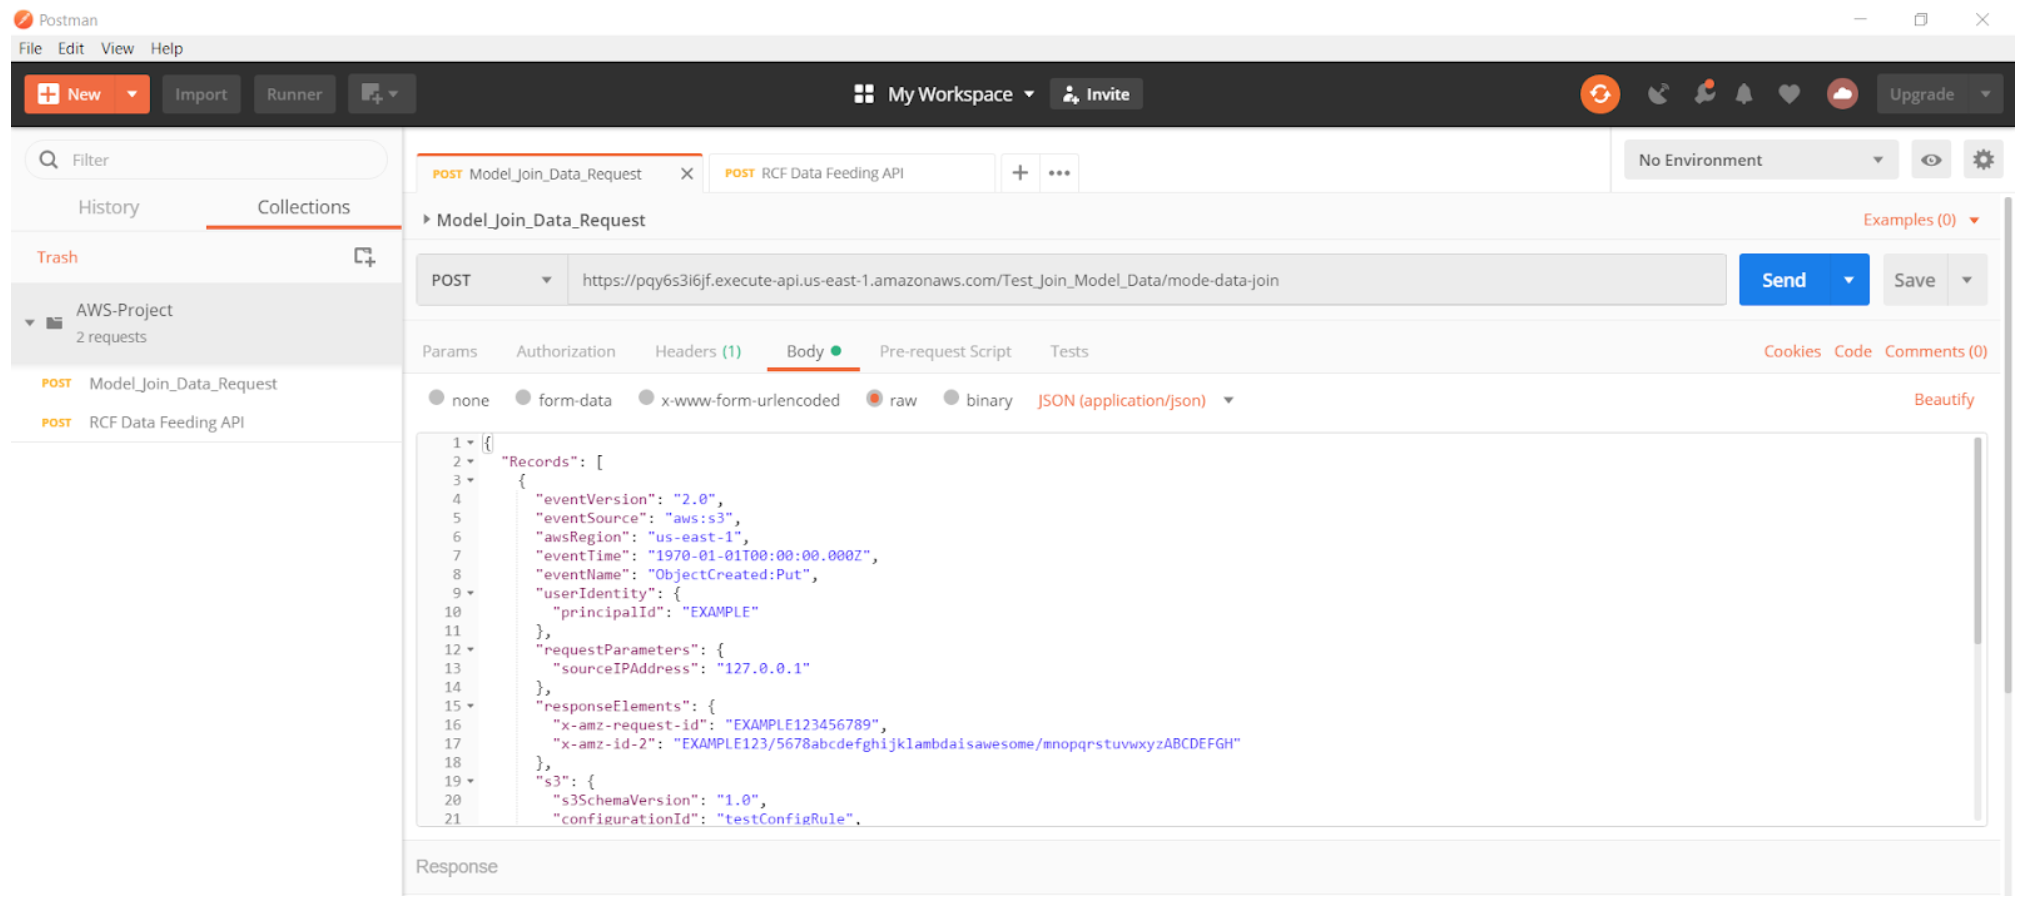
\includegraphics[width=1\textwidth]{images/api-gateway.png}
    \caption{Example of API Gateway using Postman}
    \label{fig:api_gateway}
\end{figure}

\textbf{Model\_Data\_Join.py} can be found in the \verb|/lambdas| folder in the github repository.
This function main job is sending data to the model. Using a specific prefix directory, we let the function access our data bucket and look up all keys inside it. The sent data is going to be tested for anomalies, so we couldn't just send a VPC-FlowLog to the model. Instead, we created a file reader, where we read all the keys inside the directory (Keys are FlowLogs), we parse a small json file with index + number of lines inside them. Number of lines = number of request inside each single Flowlog. This was the most convenient way to send requests number to the model using FlowLogs (Fig. \ref{fig:lambda_key_reader}).

\begin{figure}[h!]
    \centering
    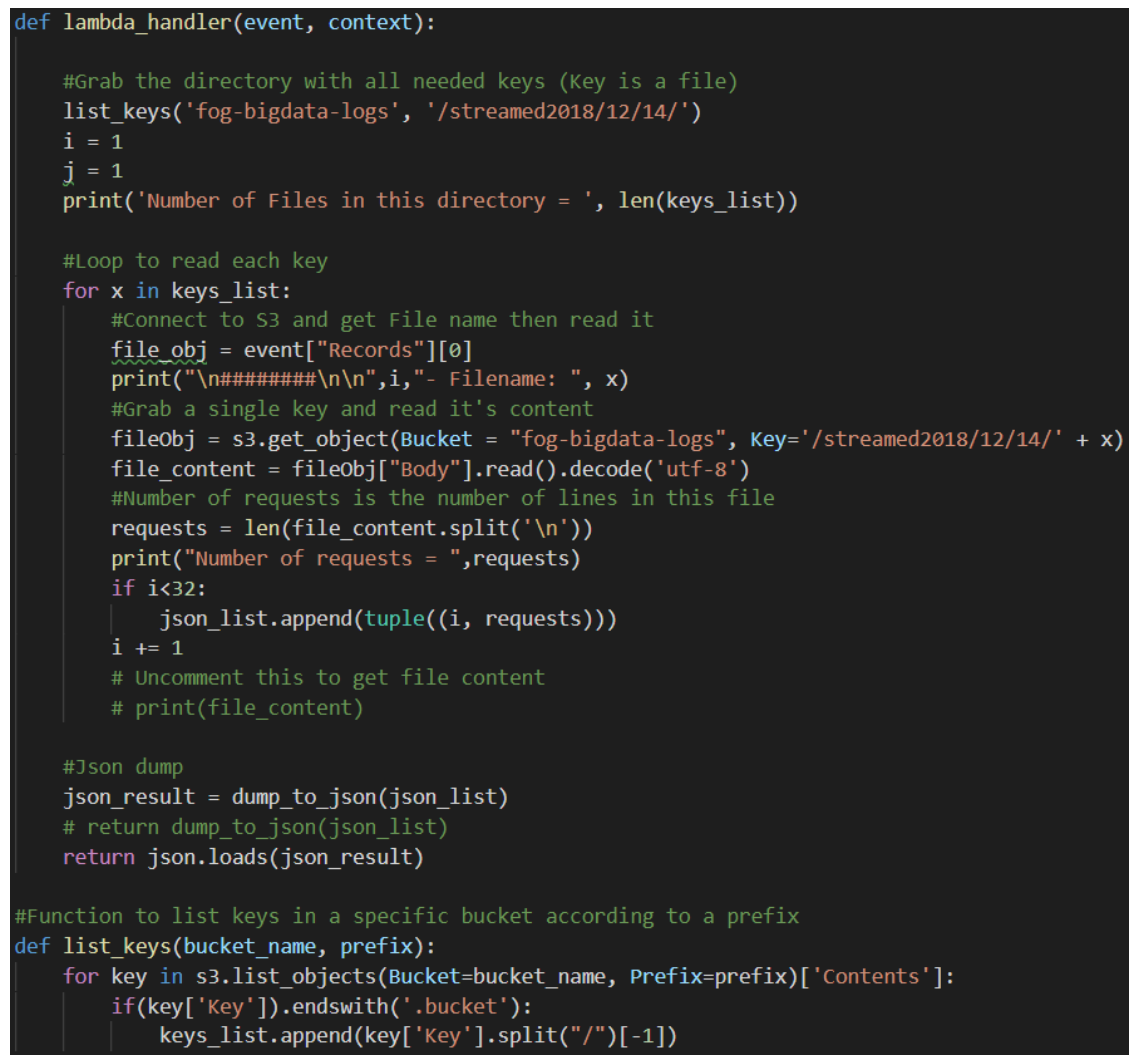
\includegraphics[width=1\textwidth]{images/lambda-key-reader.png}
    \caption{Lambda Key Reader}
    \label{fig:lambda_key_reader}
\end{figure}

After the data has been parsed from the keys, we get a list, converted to a JSON file later dumped inside the bucket to keep as a history of data that has been used. 
This process also involves sending the data to the model, after parsing it to json format. We used the invoke method provided from AWS to achieve this. The method takes another lambda function \verb|AnomalyDetection| and the data file as a variable \verb|(json\_data)|. Below you can see the code for this.

\begin{figure}[h!]
    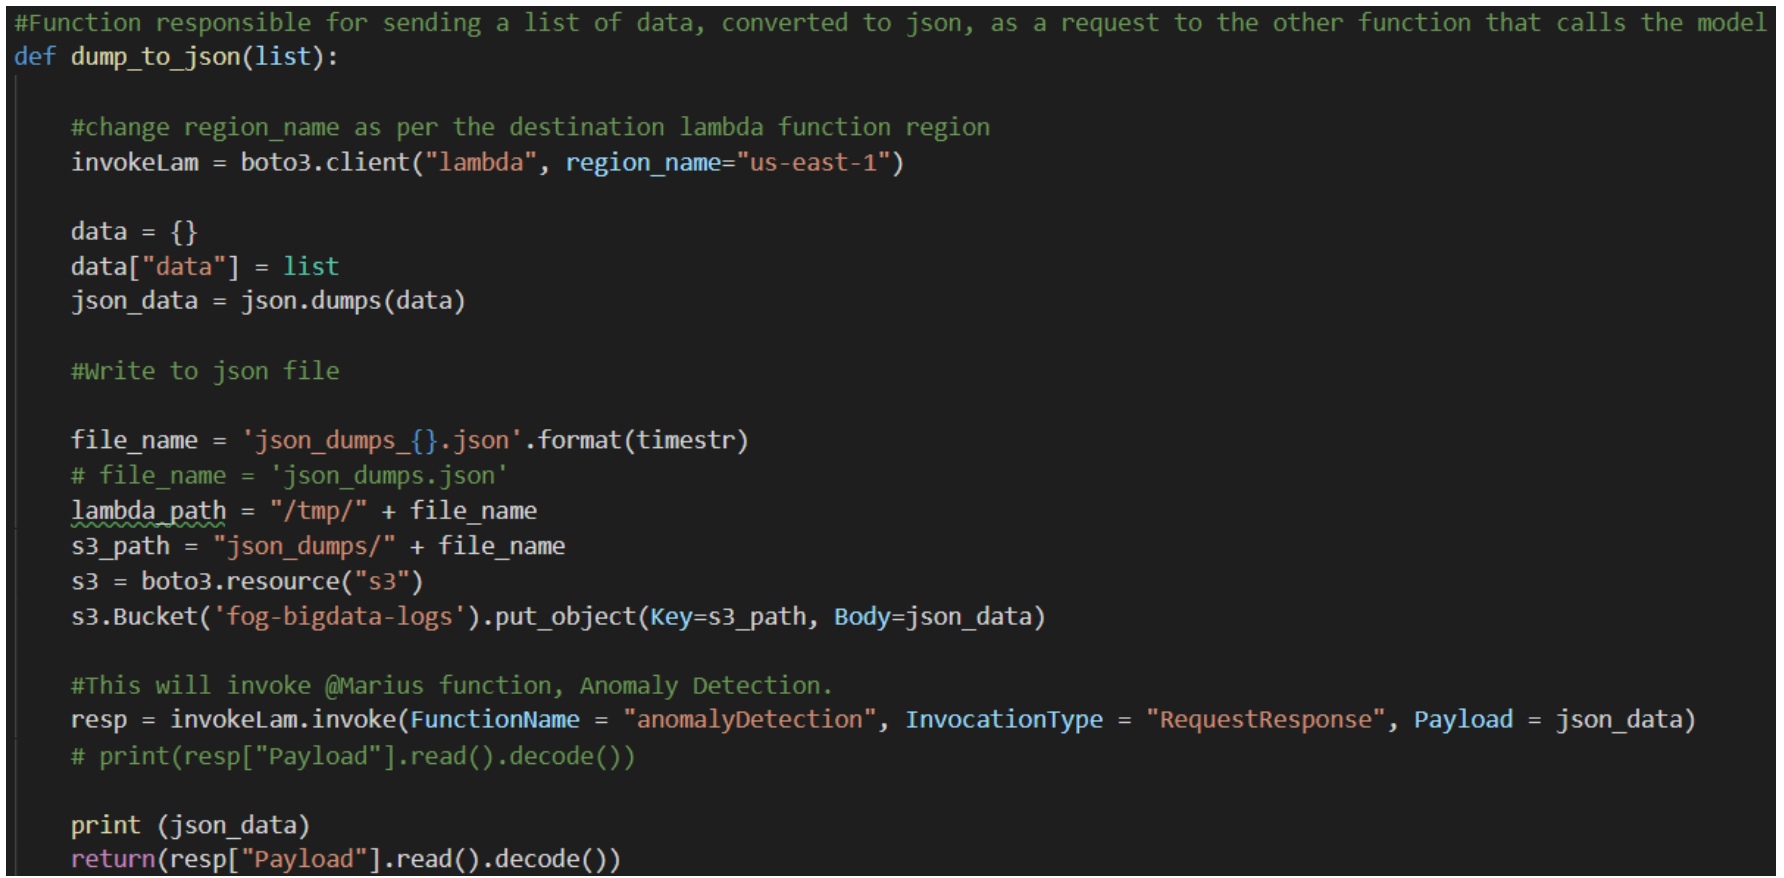
\includegraphics[width=1\textwidth]{images/json-dump-code.png}
    \caption{JSON Dump code}
    \label{fig:json_dump_code}
\end{figure}

After sending the data to \verb|anomalyDetection| lambda, we parse the event back to CSV format for the model to understand it. We separate each value by a new line. Result from the model is then parsed and passed through a prediction method to give us which values where TRUE as anomalies. This result is sent to our AWS channel using an SNS topic (arn:aws:sns:us-east-1:746022503515:api-test) created to queue all notifications.
\begin{figure}[h]
    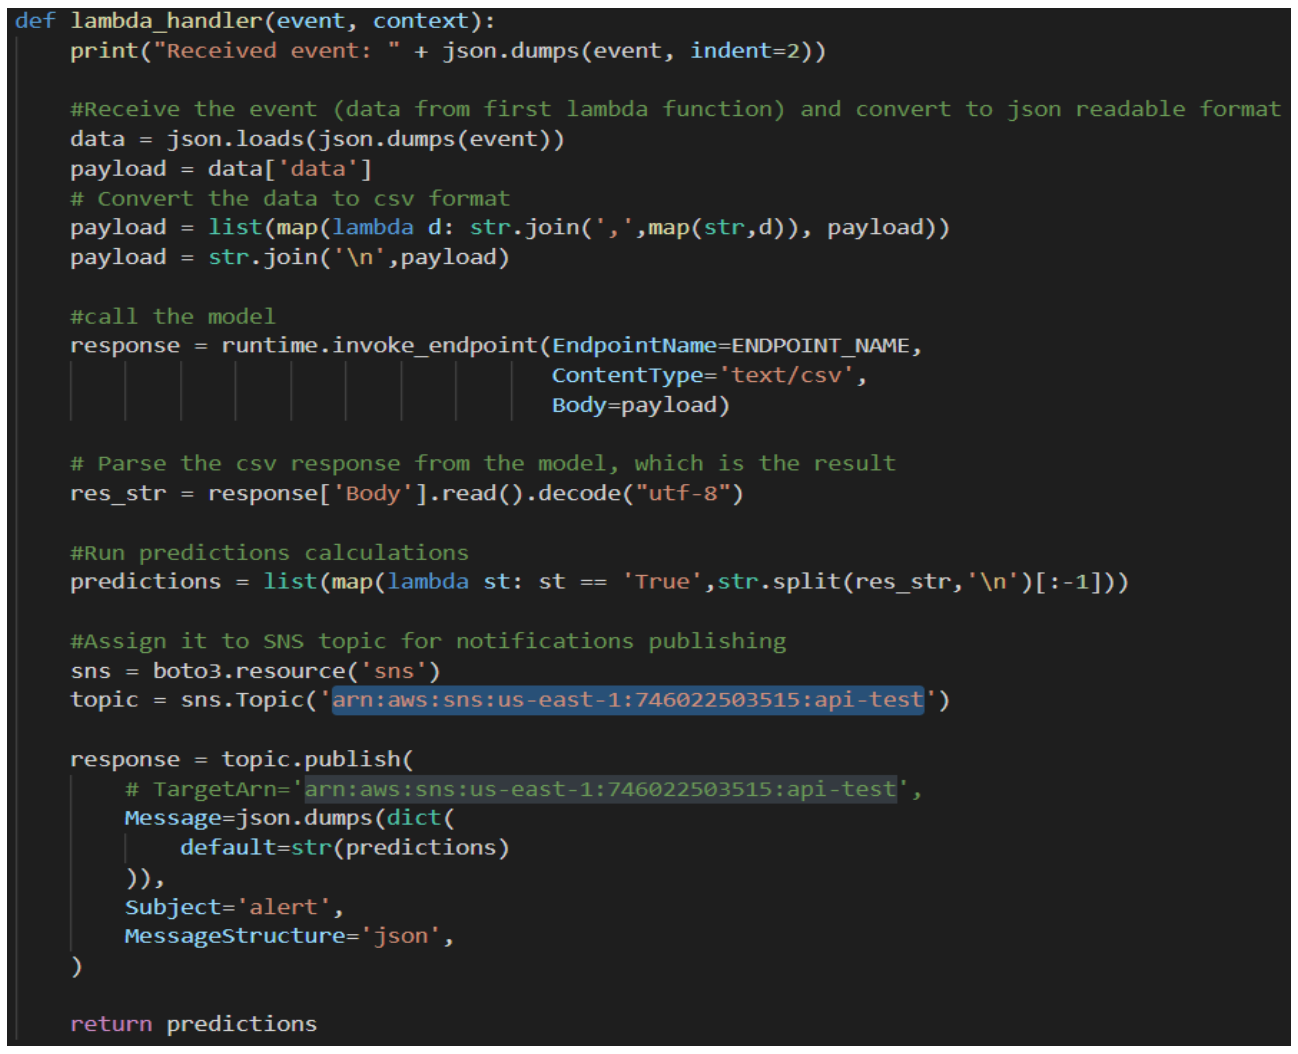
\includegraphics[width=1\textwidth]{images/lambda-precistion.png}
    \caption{Lambda precision}
    \label{fig:lambda_precision}
\end{figure}
Since this was our first demo, we didn't enable automatic triggering with every new data file, instead, we created test events with the needed buckets and triggered them manually. To make it work properly, you just need Flow-Logs inside the directory (as shown in Fig. \ref{fig:lambda_precision}). 
            

\subsection{RCF (Fixed Data)}
RCF Random Cut Forest is unsupervised algorithm for detecting anomalous data points within a dataset and was used in a SageMaker as our second trial model. \\

The data connection with this model was a bit more complex; even though the model took normal json format, we had to separate the values and parse the results several times to make a clean execution. The model takes a list of data points, then returns back a result which is \verb|Scores\_Array|. These scores have to be calculated again using a specific function to get the anomalies (above or below the RCF threshold). Based on those values, we trigger an alert that sends notifications to our channels. However, the procedure also was changed to almost fully automatic! We added a trigger to the functions \verb|rcf-sagemaker-testdata| with a suffix (.csv) and objectCreated event over an S3 bucket, which triggers the whole work-flow by itself. An API gateway \verb|RCF\_API| was also created for the same purpose of our first model.\\

Two S3 buckets were involved in this process, \verb|rcf-sagemaker-finished| and \verb|rcf-sagemaker-testdata|. A small overview of the work-flow is described below:
\begin{enumerate}
\item Make sure the model endpoint is working properly (preliminary checks per usual)
\item Upload data to 1 bucket \verb|rcf-sagemaker-testdata|
\item This upload to S3 bucket automatically triggers using SNS topic all subscribed lambda functions.
\item 2 functions are then triggered. The data from S3 bucket is read, prepared and send to the model. Since the model is already feed with a new data, the input data from the initial S3 bucket are moved to the finished sets to \verb|rcf-sagemaker-finished| S3 bucket.
\item Results and especially the anomaly detection, trigger the notification functions which inform the user about the anomalies.
\end{enumerate}

\textbf{Used functions}
The whole process involved 2 functions, \verb|RCF\_Data\_Join\_SageMaker.py| and \verb|RCF\_Anomaly\_Model\_2.py|. The first function is triggered by file upload to the S3 bucket and reads uploaded data. After parsing the data the function sends the filtered data to the second function, where we call the model for analysis.
All policies, notes, used variables, endpoint names etc. can be found in github repository under \verb|Notes.txt|.
The function reads all files in the S3 bucket and lists them for logging purposes. Once we upload a file, it separates it into 2 versions. The data is usually DATE SCORE format.
So we create 2 lists, 1 with both values and 1 that has only the scores data. We do this because we want to preserve the date as time-stamp history for the model.
Once we have the parsed data, the process of sending this data starts. The smart thing about this is that we used AWS functions to clear our buckets. The data gets sent from \verb|rcf-sagemaker-testdata| bucket to \verb|rcf-sagemaker-finished| bucket, with the name changed to include time of the data testing and date as shown in the Fig. \ref{fig:rcf_data_movement}.\\

\begin{figure}[h]
    \centering
    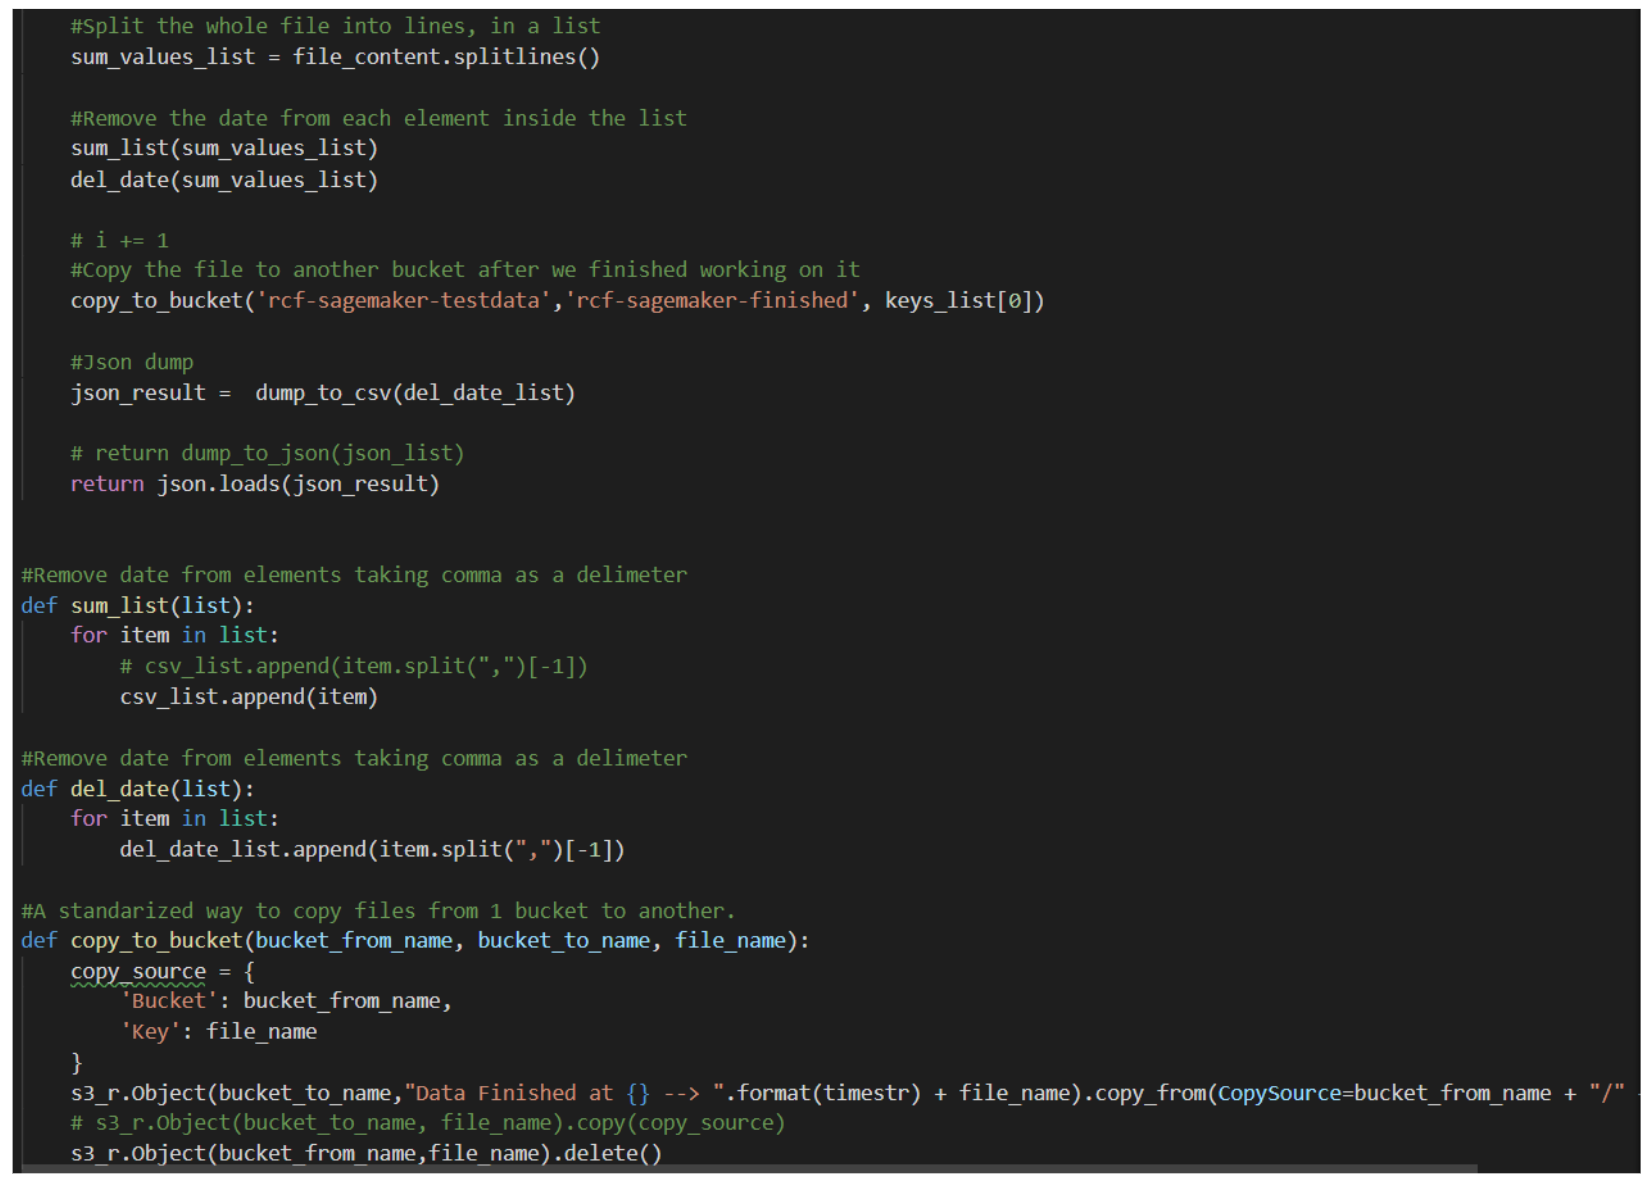
\includegraphics[width=1\textwidth]{images/rcf-data-movement.png}
    \caption{The moving of data from testing buckets to finished testing data}
    \label{fig:rcf_data_movement}
\end{figure}

We then proceed to call \verb|dump\_to\_csv|, where we send the data to the model including the date time-stamp, and also create a \verb|csv\_dump| folder inside the finished bucket for testing and debugging purposes.\\

The model function, \verb|RCF\_Anomly\_Model\_2.py| is then invoked with the needed json data. 
\begin{figure}[h]

    \centering
    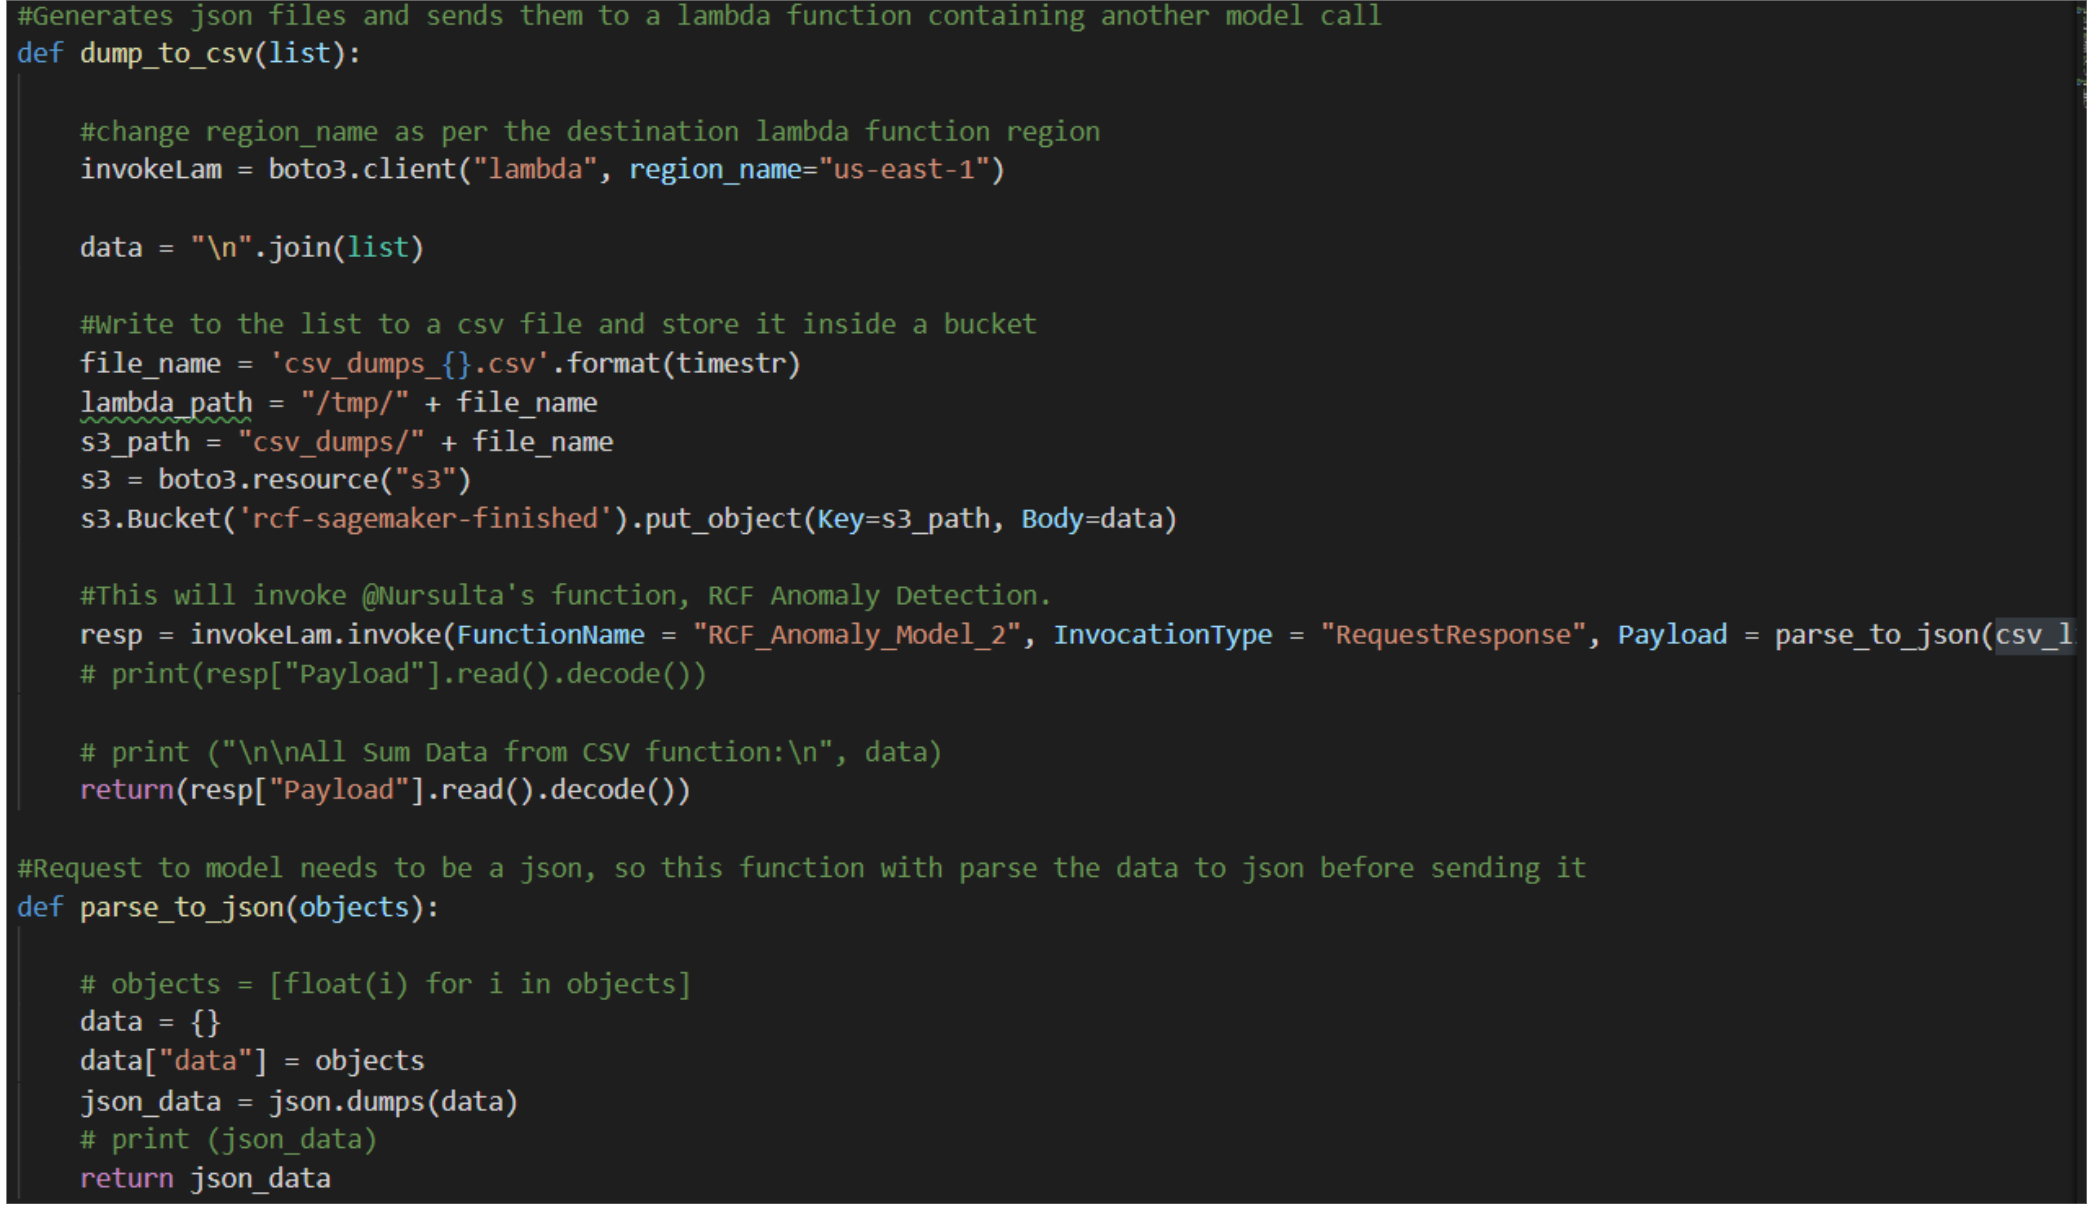
\includegraphics[width=1\textwidth]{images/json-generator.png}
    \caption{Invoking RCF-Anomly-Model-2.py}
    \label{fig:json_generator}
\end{figure}
And as a result of some time consuming calculations in this function, we had to make the run-time of lambda up to 3 minutes to avoid any unwanted failures.\\
After the json event is received, we parse it back to the correct csv format and send it to the model using \verb|invoke\_endpoint| method. The result is a huge CSV response with all the values we need to calculate with RCF for anomalies.\\
The final cut-off score is calculated with the following equations:
\begin{figure}[h]
    \centering
    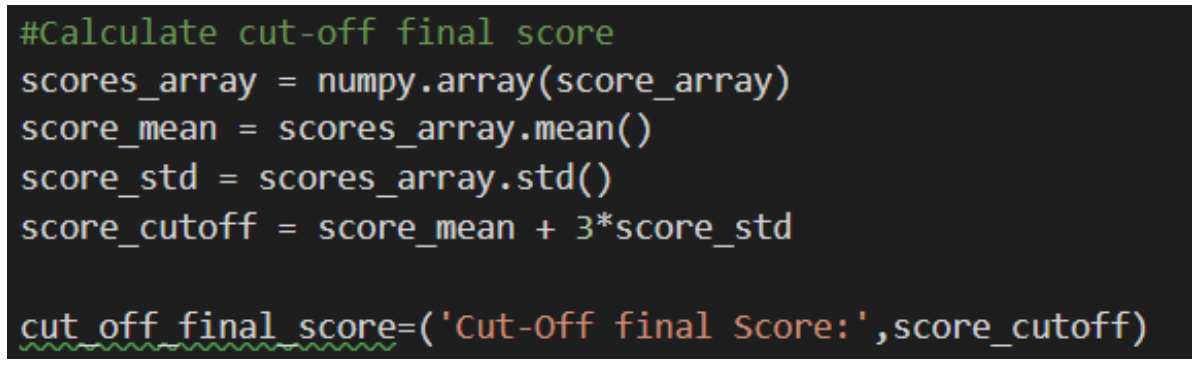
\includegraphics[width=1\textwidth]{images/cutt-off-calculator.png}
    \caption{Cut-off score calculator}
    \label{fig:cut_off_calculator}
\end{figure}
Based on the calculated RCF Threshold we compare the values based on the input data and mark those over the threshold level as an anomalies. Once anomaly is detected notification process starts.\\
\begin{figure}[ht]
    \centering
    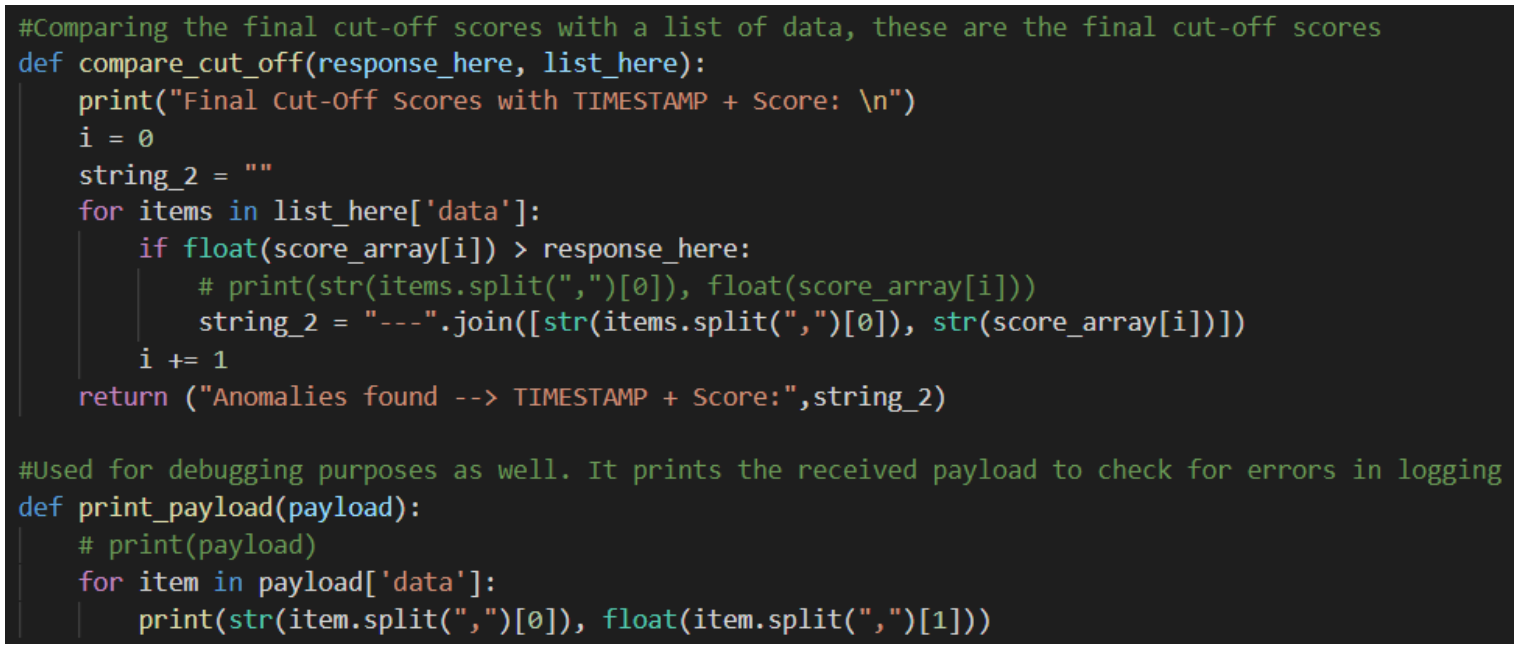
\includegraphics[width=1\textwidth]{images/cutt-off-comparison.png}
    \caption{Cut-off comparison}
    \label{fig:cut_off_comparison}
\end{figure}
Once we have everything calculated and compared, the results are sent to another part of the function where we start sending alerts and notifications. For this we created a specific Slack App \& another function that handles all the notifications. This can be found in a detailed section down below under Notifications Functions.\\

The graph generation was a bit of a complicated manner, since we can’t send direct images from lambda to slack without doing a workaround. We had to store the results in a memory buffer, and read that buffer to send it. Notifications being sent had the anomalies, a graph with the data + threshold + anomalies detected in a detailed form.\\

Using panda, we saved data points in an X (\textbf{Date Stamp}) and Y (\textbf{Scores}) lists after reading the file from lambda’s tmp directory and generate the plot.
\begin{figure}[h]
    \centering
    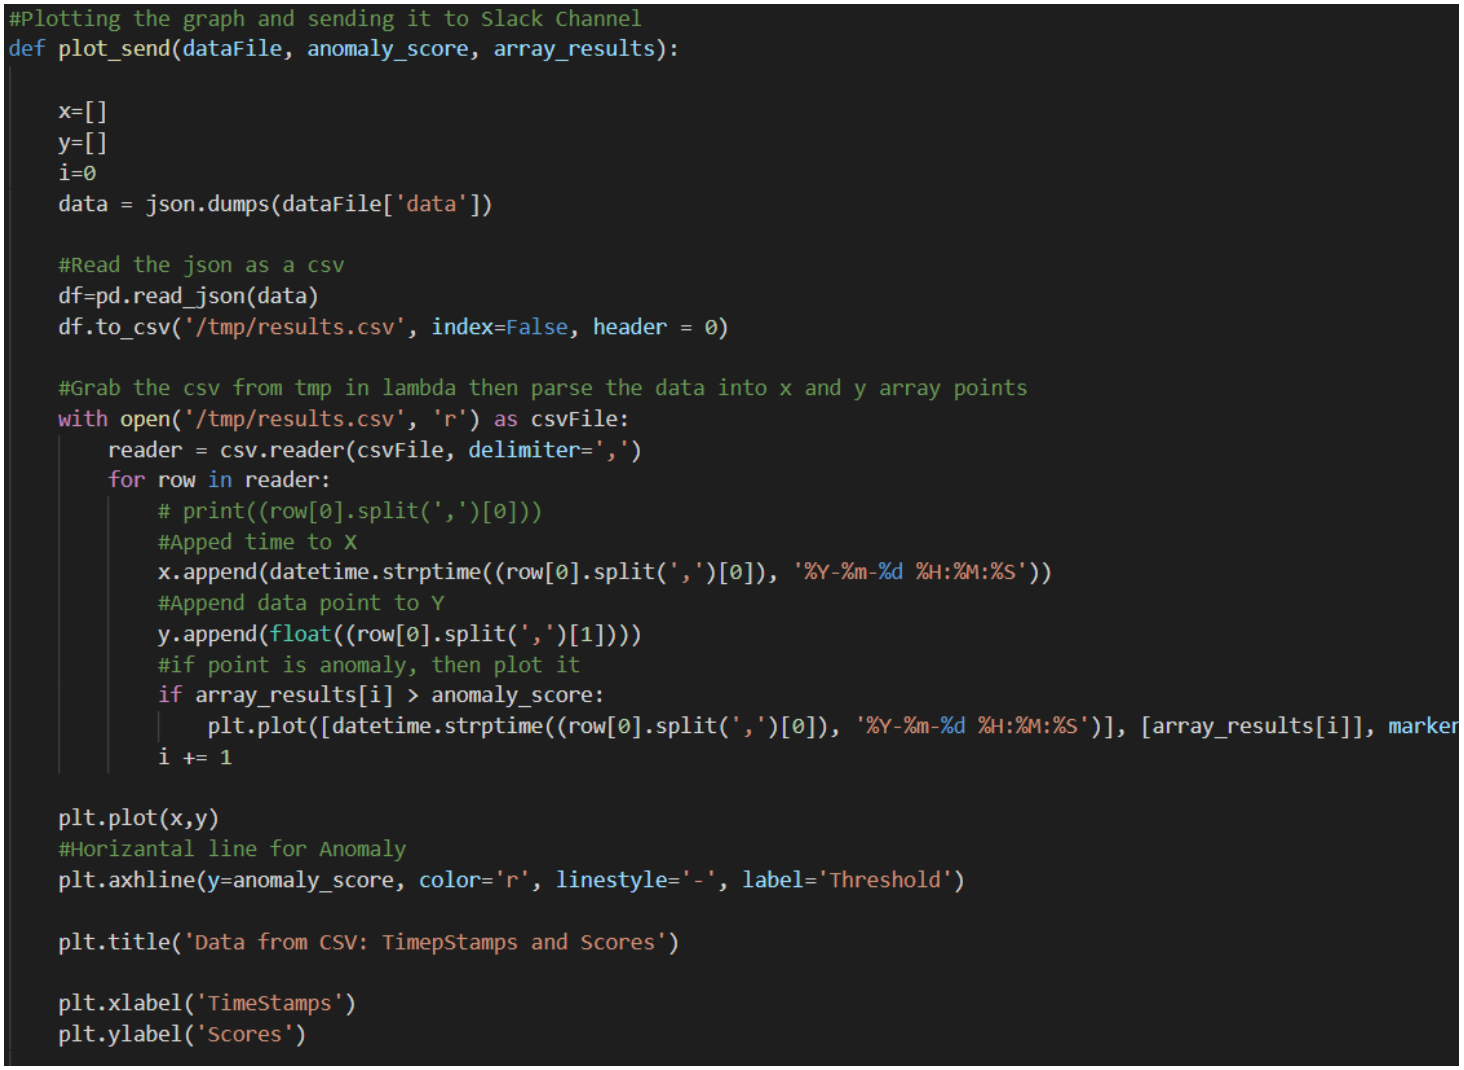
\includegraphics[width=1\textwidth]{images/graph-plotting.png}
    \caption{Plotting the anomaly graph}
    \label{fig:graph_plotting}
\end{figure}
Then sent to slack with a special \verb|payload\_2 param|, that holds our channel name, title and some other needed variables for better readability. In general, this all happens in an automatic form.